\section[Contributing to the Question Pool]{Contributing}

\begin{frame}
  \frametitle{Contributions via the HPCCF-Wiki}
  \centering
  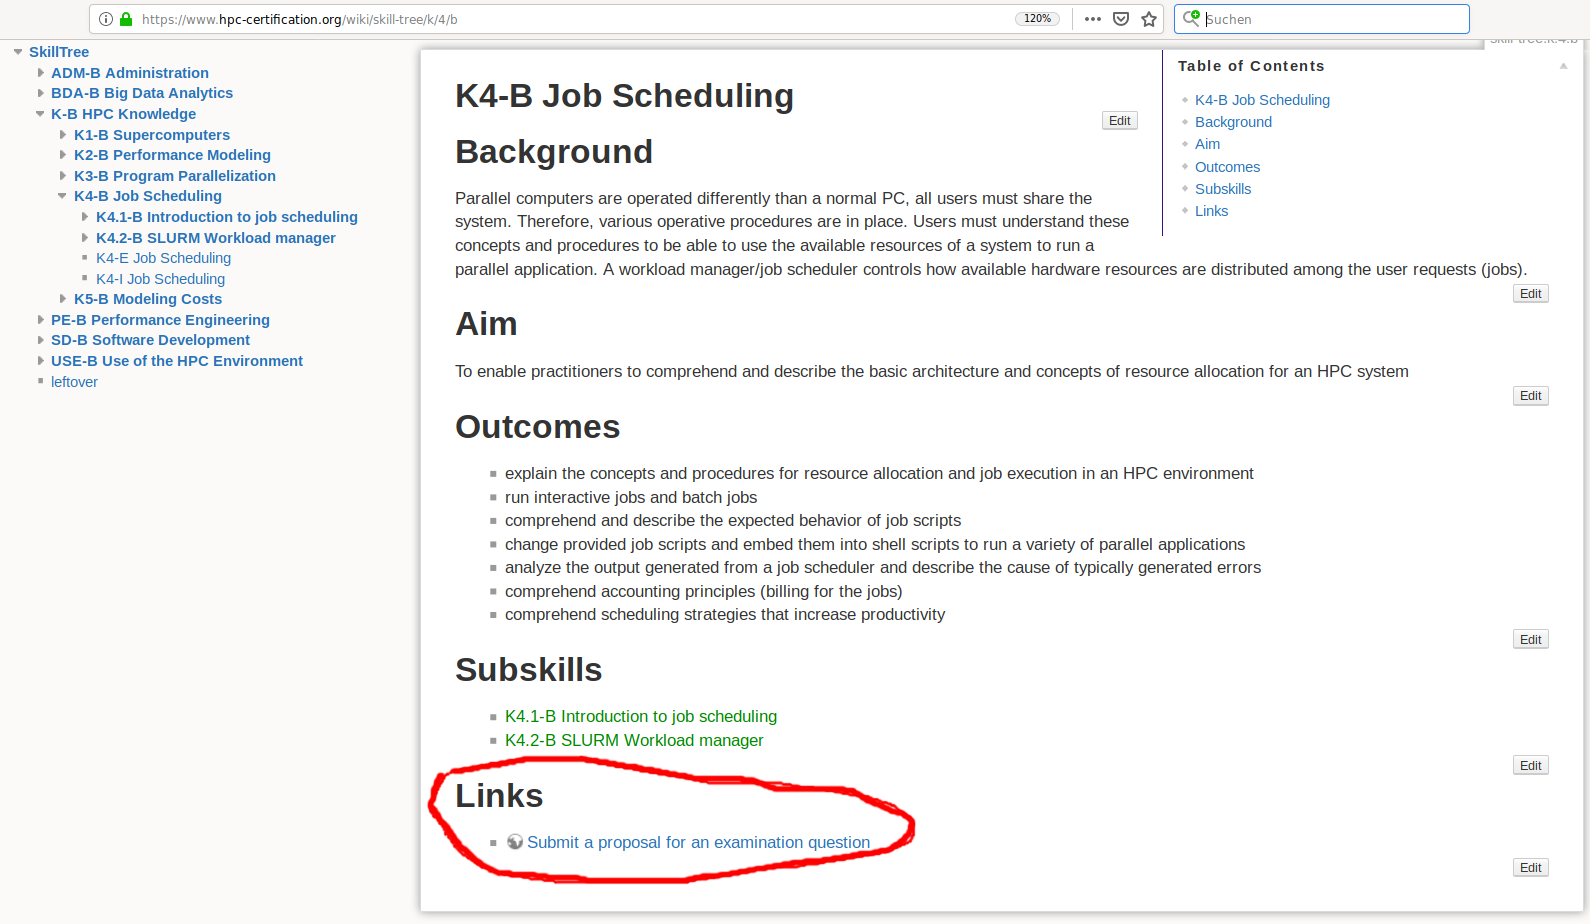
\includegraphics[width=0.8\textwidth]{images/contribution}
\end{frame}


\begin{frame}
  \frametitle{Contributions via the HPCCF-Wiki II}
  Each \lhref{https://www.hpc-certification.org/wiki}{HPCCF wiki} page contains a link. It leads to a little form asking for:
  \begin{itemize}
   \item contact mail
   \item to select a learning objective from a pre-formatted list
   \item to supply the question you thought of
   \item and (in case of a multiple choice question) the possible answers.
  \end{itemize}
  \pause
  \task[Evaluation Process]{Now, HPCCF-member evaluate the submitted question. If approved, it will be formatted and merged into the pool of questions for the choosen topic / skillset.}
\end{frame}


\begin{frame}{Certification: Assessment Prototype}
		\begin{enumerate}
			\item User takes multiple-choice test online (any time!)
			\begin{itemize}
				\item A combination of JavaScript and a web service
				\item System selects number of questions randomly from a pool
					\begin{itemize}
						\item By submitting questions the related usage-allowance is granted to HPCCF
					\end{itemize}
				\item In case of sufficient numbers the system draws from a pool of different possible answers (MCQ-case).
			\end{itemize}
			\item Choices are submitted to the web server
			\item \textit{Manual approval} of the result
			\item Automatic creation of certificate and returned by email
			\begin{itemize}
							\item Permanent computer-verifiable proof is created about certification of skills
							\begin{itemize}
								\item Return a text version with GPG signature
								\item Return a link that can be verified on hpc-certification.org
							\end{itemize}
			\end{itemize}
			\item Privacy: minimize information stored on servers, keep some for statistics
			\item Includes some measure to prevent cheating and brute forcing (e.g., delay)
		\end{enumerate}
\end{frame}

\begin{frame}[fragile]{Certification: Certificate}
\begin{columns}
	\column{0.6\textwidth}
	\begin{block}{Text representation}

		\scriptsize
		\begin{verbatim}
-----BEGIN PGP SIGNED MESSAGE-----
Hash: SHA512
HPC Certification Forum Certificate
This text confirms that "Jane Doe" has
successfully obtained the certificate
"HPC driving license" (id: 1) at 02/2019.
Verification URL: https://hpc-certification.org/[...]
-----BEGIN PGP SIGNATURE-----
[...]
-----END PGP SIGNATURE-----
		\end{verbatim}
	\end{block}

\column{0.4\textwidth}
	\begin{block}{Certificate}
		\medskip
		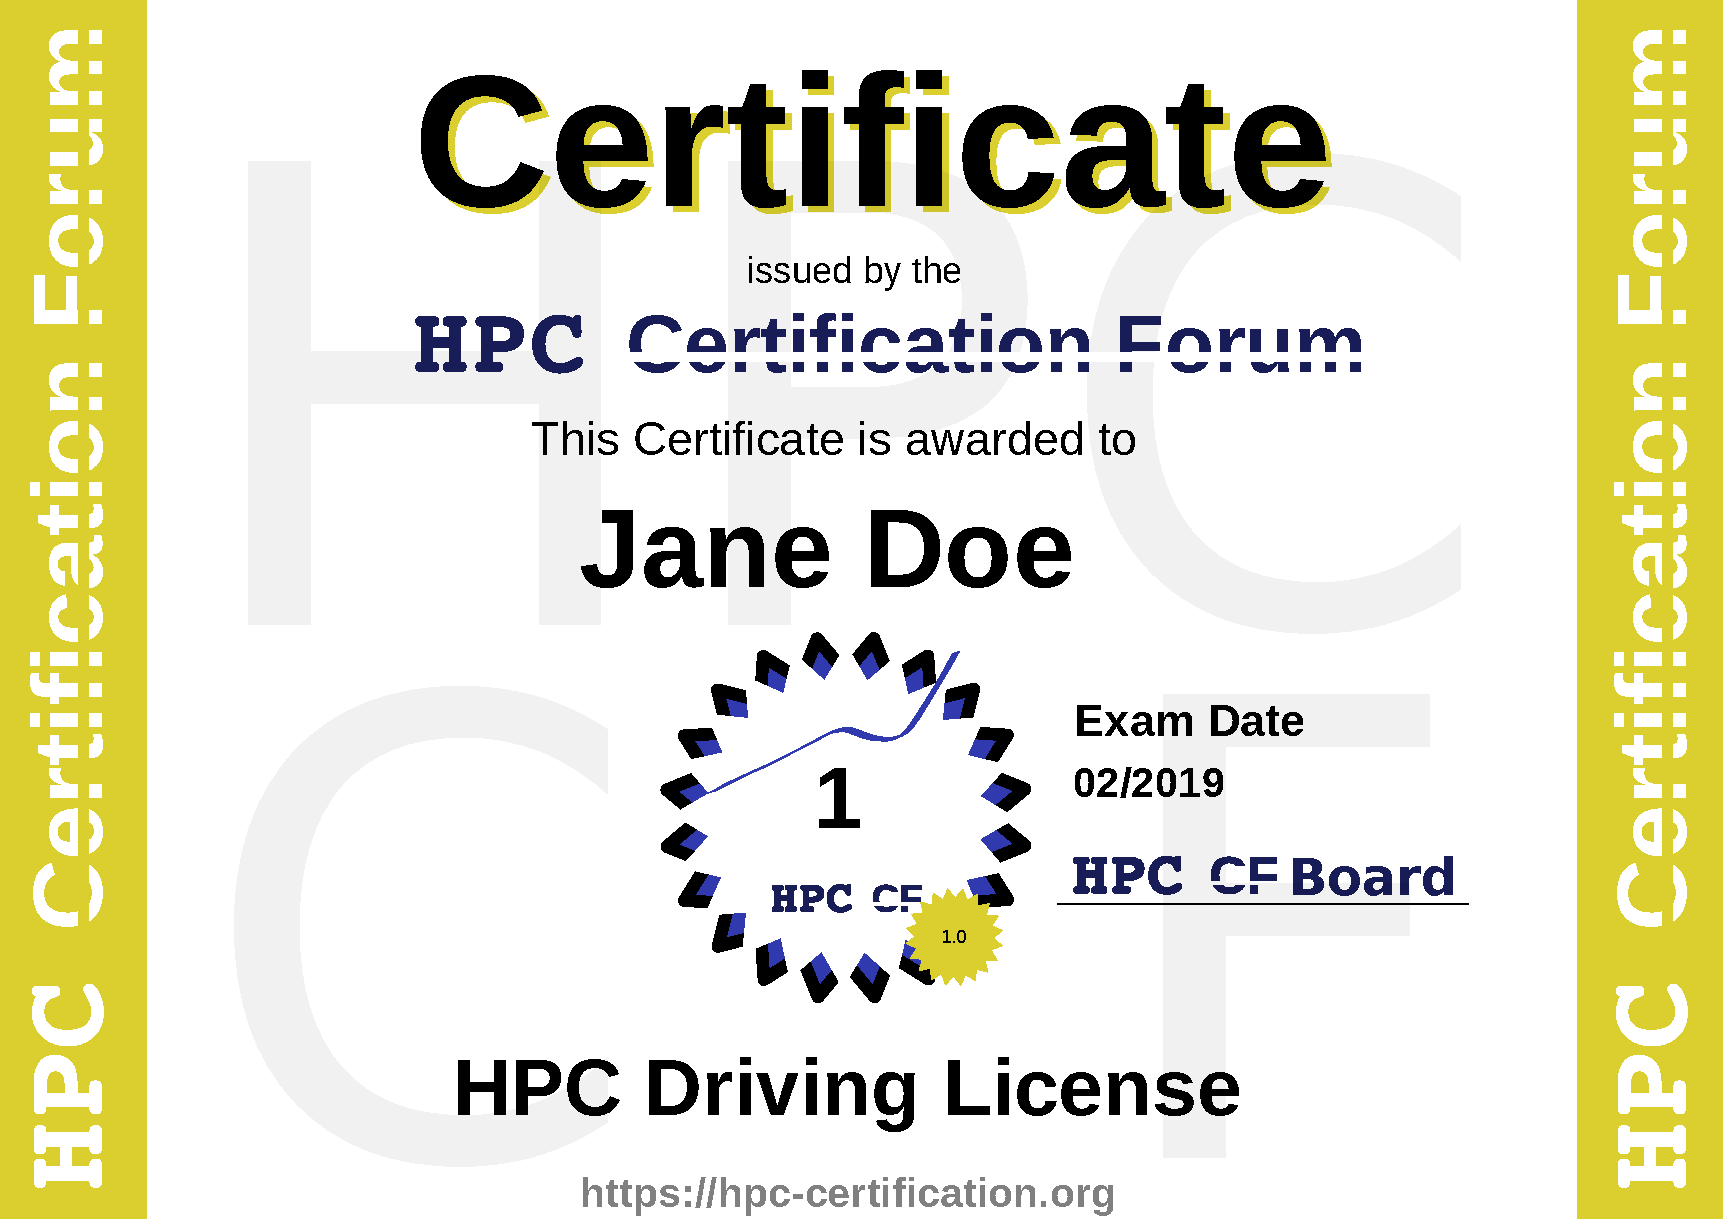
\includegraphics[width=\textwidth]{jane-doe}
	\end{block}
\end{columns}
\end{frame}
